% Created 2016-02-18 Thu 09:28
\documentclass[12pt,a4]{article}


\usepackage{fixltx2e}
\usepackage{graphicx}
\usepackage{longtable}
\usepackage{float}
\usepackage{wrapfig}
\usepackage{rotating}
\usepackage[normalem]{ulem}
\usepackage{amsmath}
\usepackage{textcomp}
\usepackage{marvosym}
\usepackage{wasysym}
\usepackage{amssymb}
\usepackage{hyperref}
\usepackage{minted}
\usepackage{fontspec,xltxtra,xunicode}
\setmainfont[Scale=0.8]{Palatino Linotype}
\setsansfont{Fira Sans}
\setmonofont[Scale=0.8]{Inconsolata}
\newfontfamily\myunicodefallback{Cambria}
\usepackage{polyglossia}
\setmainlanguage{italiano}
\usepackage{geometry}
\hypersetup{colorlinks,linkcolor=,urlcolor=links}
\definecolor{links}{HTML}{0086F7}
\setlength\columnsep{0.75cm}
\author{Vittorio Zaccaria}
\date{\today}
\title{Response time charts}
\hypersetup{
  pdfkeywords={},
  pdfsubject={},
  pdfcreator={Emacs 24.5.1 (Org mode 8.2.10)}}
\begin{document}

\maketitle
\tableofcontents


\section{Osservazioni/Da capire}
\label{sec-1}

\begin{itemize}
\item Come mai il carico misto non e' come tutti gli altri
\item Aumentare il numero di core non cambia la media ma sembra irrobustire le campane del service time
\end{itemize}

\section{Response time vs payload size}
\label{sec-2}

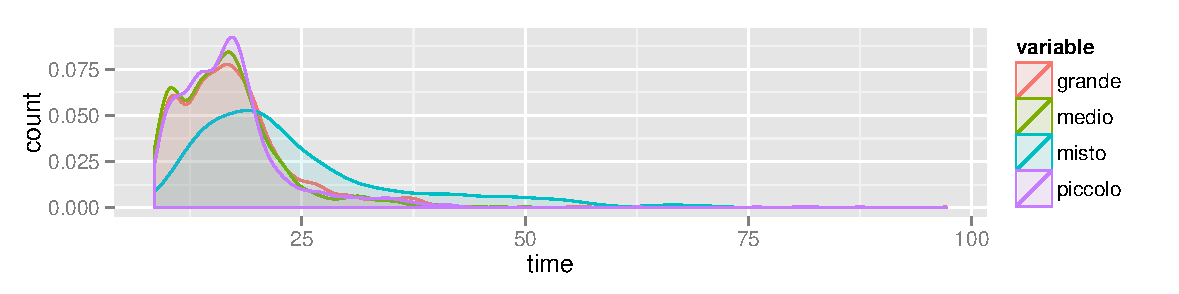
\includegraphics[width=.9\linewidth]{figures/response-time-vs-payload.pdf}

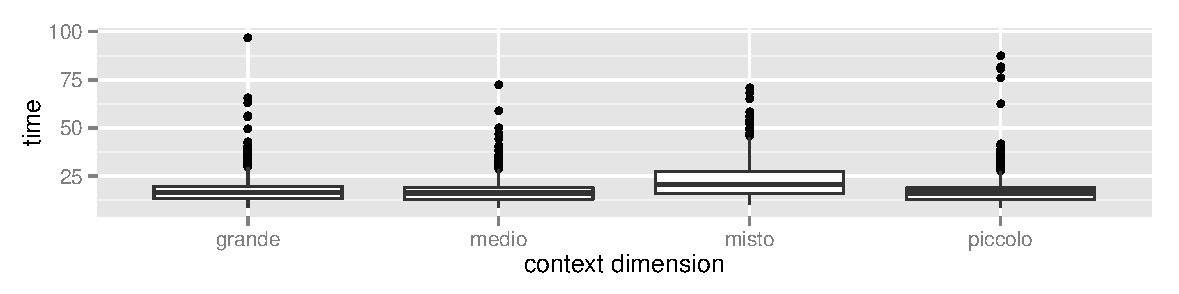
\includegraphics[width=.9\linewidth]{figures/response-time-vs-payload-boxplot.pdf}

\section{Response time vs services}
\label{sec-3}

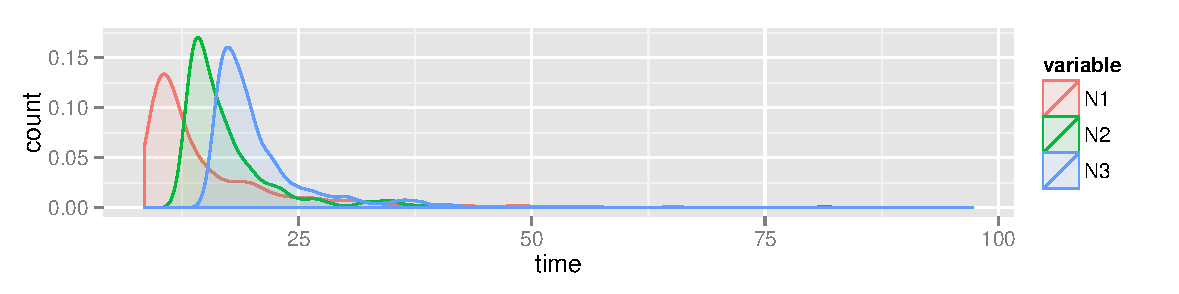
\includegraphics[width=.9\linewidth]{figures/response-time-vs-numsrvc.pdf}

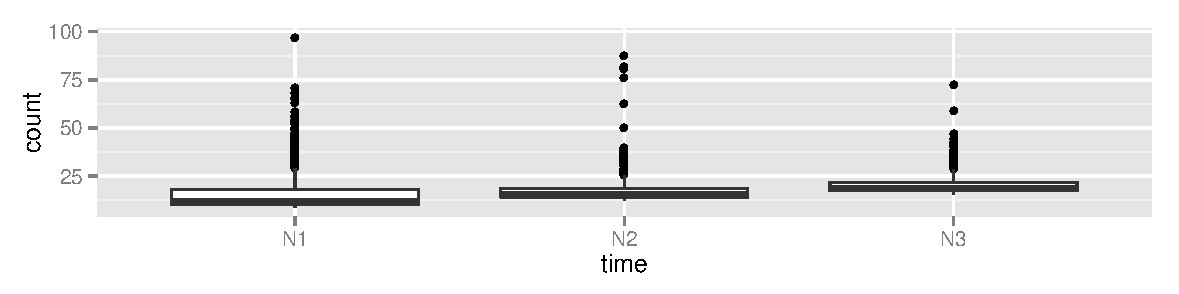
\includegraphics[width=.9\linewidth]{figures/response-time-vs-numsrvc-box-plot.pdf}

\section{Response time vs cores}
\label{sec-4}

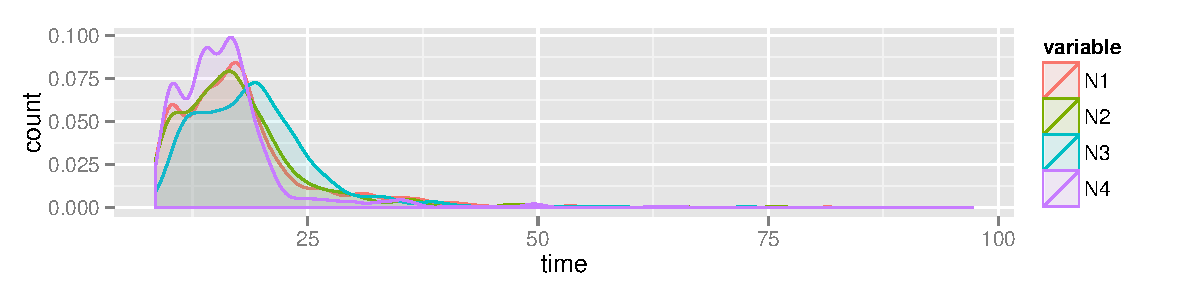
\includegraphics[width=.9\linewidth]{figures/response-time-vs-core.pdf}

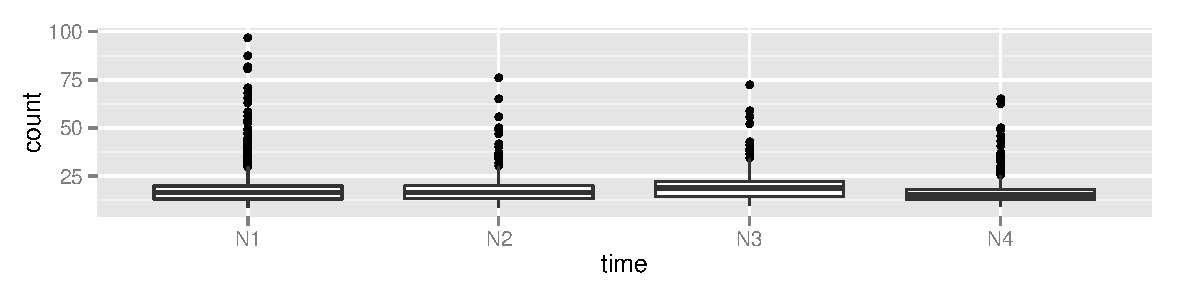
\includegraphics[width=.9\linewidth]{figures/response-time-vs-core-box-plot.pdf}

\section{Response time vs ram}
\label{sec-5}

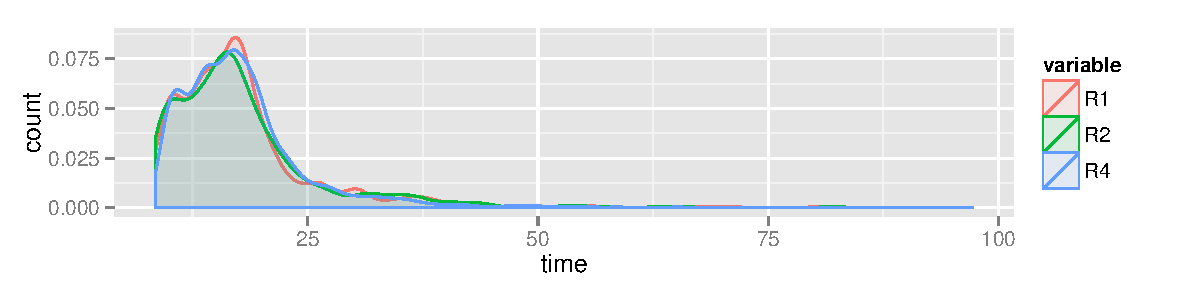
\includegraphics[width=.9\linewidth]{figures/response-time-vs-ram.pdf}

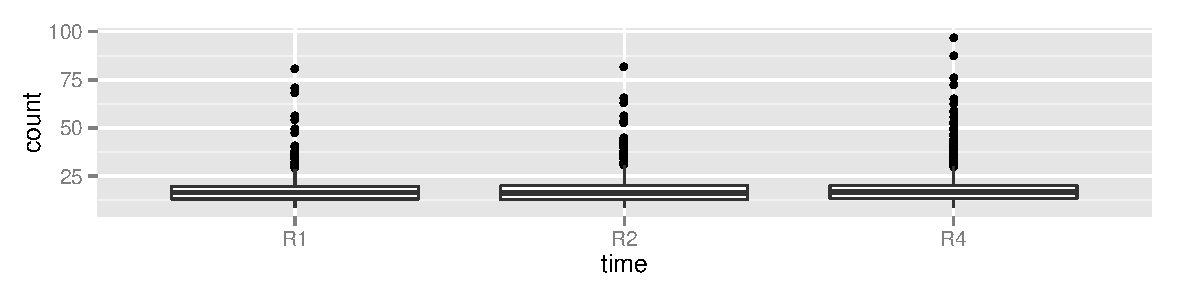
\includegraphics[width=.9\linewidth]{figures/response-time-vs-ram-box-plot.pdf}
% Emacs 24.5.1 (Org mode 8.2.10)
\end{document}